In this report, the main project choices and the results for structural ensemble PED00020 of measles virus nucleoprotein (for its five deposited ensembles) are reported.

\section{Task 1}\label{sec:task1}
\graphicspath{ {./figures/} }

The goal of the first task is to implement a tool to identify conformational relationships within a single ensemble. The input is a set of files, each containing the PDB structure of one ensemble. From now on, they will be analyzed separately and relationships between the conformations within an ensemble are identified analyzing the model structural features. 


\subsection{Single conformation features}

Firstly, for each conformations, the software extracts the structural features and saves them into a unique dictionary:
\begin{itemize}
\item Radius of gyration of the structure: it is computed using the coordinates of each atom and their barycenter.
\item Relative accessible surface area (ASA) for each residue: it is computed thanks to DSSP; note that the values obtained for the conformations within an ensembles are equal. It may happen that the DSSP does not return the ASA value for each residue: for this limitation, a check on the array dimension and, if needed, a zero-padding are performed. 
\item Secondary structure for each residue: they are determined thanks to the Ramachandran regions associated with Phi and Psi angles of the each residue. For the first and last residue, for which the value is not computable, `-' is inserted. For a simpler store and data analysis, each obtained value is converted into the correspondent integer value reported in table \ref{tab:ss}. 
\item Distance matrix: it computes the pairwise distances between each pair of residues.% For a simpler store and data analysis, each obtained value is converted into the correspondent integer value reported in table x.
\end{itemize}

\begin{table}[H]
\begin{center}
\begin{tabular}{lr}
% FIRST ROW
\textbf{Secondary Structure} & \textbf{Int}\\
\hline
- & 0\\
\hline
Beta-sheet & 1\\
\hline
Polyproline I-II & 2\\
\hline
Alpha-helix & 3\\
\hline
Left-handed Helix & 4\\
\end{tabular}
\end{center}
\caption{Conversion for Secondary Structur values}~\label{tab:ss}
\end{table}



\subsection{Representative conformations} 
In order to extract the representative conformations, the software clusters the models within a single PED exploiting KMedoids approach and a custom metric function. The proper number of clusters is set thanks to Silhouette measure. 
KMedoids is exploited since it allows to use an arbitrary dissimilarity measures and the centroids are chosen between the points already present in the analyzed set. 

\medskip
The metric function uses different distance metrics to measure the distances between the features calculated at the previous point. It takes in input the feature vectors for two conformations and compute their distance as sum of the following partial features distances:
\begin{itemize}
\item Absolute difference between radius of gyration to understand its variation.
\item Euclidean distance of ASA vectors.
\item Distance between SS vectors using a scoring matrix accordingly to their definition and properties. The scoring matrix is reported in table \ref{tab:score}. 
\item The cosine distance between distance matrix. 
\end{itemize}

\begin{table}[H]
\begin{center}
\begin{tabular}{c|ccccc}
% FIRST ROW
& 0 & 1 & 2 & 3 & 4 \\
\hline
0 & 0 & 1 & 1 & 1 & 1\\
1 & 1 & 0 & 1 & 1 & 1\\
2 & 1 & 1 & 0 & 1 & 1\\
3 & 1 & 1 & 1 & 0 & 0.5\\
4 & 1 & 1 & 1 & 0.5 & 0\\
\end{tabular}
\end{center}
\caption{Scoring matrix Secondary Structur values}~\label{tab:score}
\end{table}


Once the representative conformations are extracted as centroids, the software plots a weighted graph, where each node is a representative model and the edge length is proportional to the distance between each pair. Moreover the edge labels are the distances between the two conformations at the extremes computed by the metric showed above. 



\begin{figure}[H]
	\begin{minipage}[b]{0.47\textwidth}
		\centering
		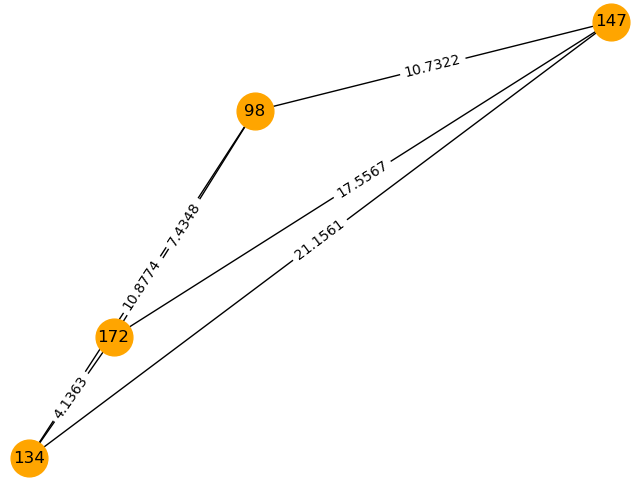
\includegraphics[width=\textwidth]{PED00020e001_graph.png}
		\caption{Graph of model 001.}
		\label{model001}
	\end{minipage}
	\hfill
	\begin{minipage}[b]{0.47\textwidth}
		\centering
		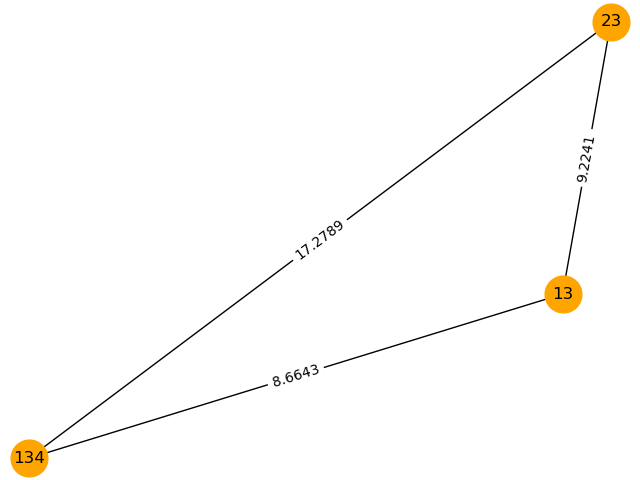
\includegraphics[width=\textwidth]{PED00020e002_graph.png}
		\caption{Graph of model 002.}
		\label{model002}
	\end{minipage}
\end{figure}
\begin{figure}[H]
	\begin{minipage}[b]{0.47\textwidth}
		\centering
		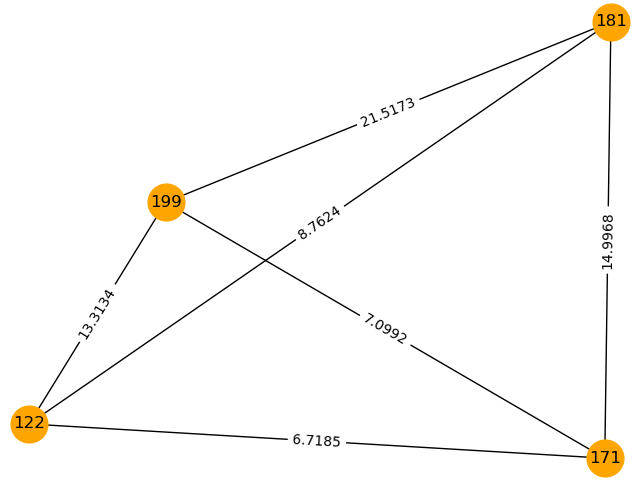
\includegraphics[width=\textwidth]{PED00020e003_graph.png}
		\caption{Graph of model 003.}
		\label{model003}
	\end{minipage}
	\begin{minipage}[b]{0.47\textwidth}
		\centering
		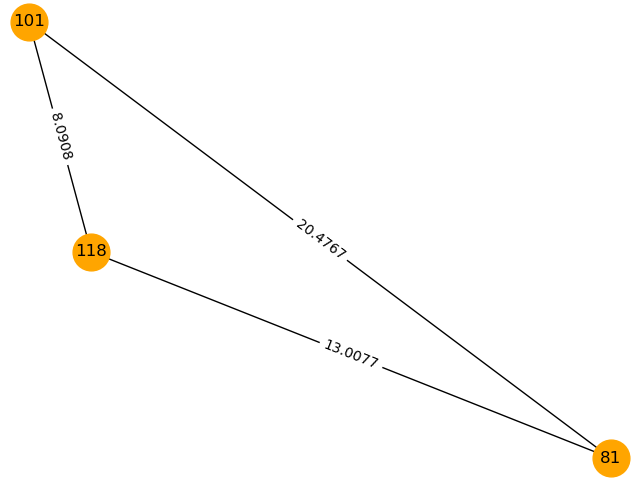
\includegraphics[width=\textwidth]{PED00020e004_graph.png}
		\caption{Graph of model 004.}
		\label{model004}
	\end{minipage}
\end{figure}
\begin{figure}[H]
	\begin{minipage}[b]{0.47\textwidth}
		\centering
		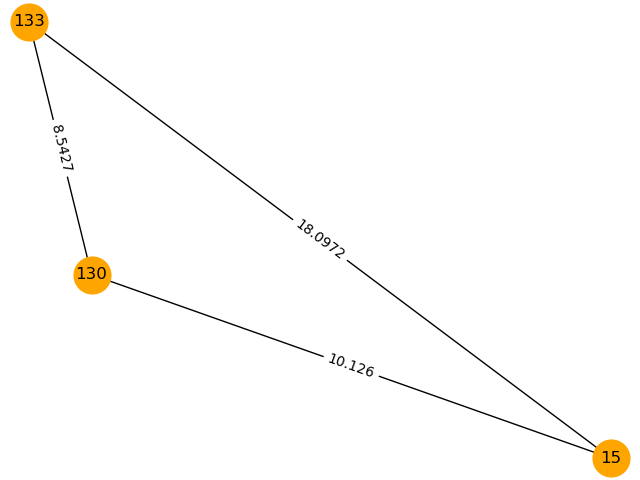
\includegraphics[width=\textwidth]{PED00020e005_graph.png}
		\caption{Graph of model 005.}
		\label{model005}
	\end{minipage}
	\end{figure}

In figures \ref{model001}, \ref{model002}, \ref{model003}, \ref{model004} and \ref{model005} the obtained graphs are reported. By running the script several times, a high results variability can be observed.
This is probably caused by the proximity of the points (represented in the features space) and the random initialization of clustering. The centroids are usually different but found in the same cardinality.



\subsection{Pymol image}
For each ensemble, the software generates a Pymol image to visualize the 3D structure of one representative conformation and the variability of each residue in terms of features (only considering the conformations extracted thanks to clustering) through the changing of the color.

We decided to generate one image for each ensemble with their representative conformations extracted within the clustering step.
As a matter of fact, generating an image representating the conformations superimposition, it would give a too messy result and not reporting important information.

\medskip
The residue variability is calculated using a metric built by us. Note that the radius of gyration is not used since it is not residual-dependent.
In order to compute the residue variability, it considers the neighbors of the residue under analysis thanks to a window of size nine to the left and to the right of the current position.

This metric returns the sum of the following partial distances:
\begin{itemize}
\item Standard deviation of ASA which evaluates the difference between the surface areas for each residual of the representative conformations of an ensemble. Then it compute the mean of the standard deviation for each residues in the window takes in consideration.
\item Distance between SS vectors pairs using the above scoring matrix accordingly to their definition and properties. It consider the residues in the current window.
\item The sum of all the variations of the distances for each residual pair in the conformation. It is computed using the cosine distance between residual pair in the window considered. 
\end{itemize}

\begin{figure}[H]
	\begin{minipage}[b]{0.97\textwidth}
		\centering
		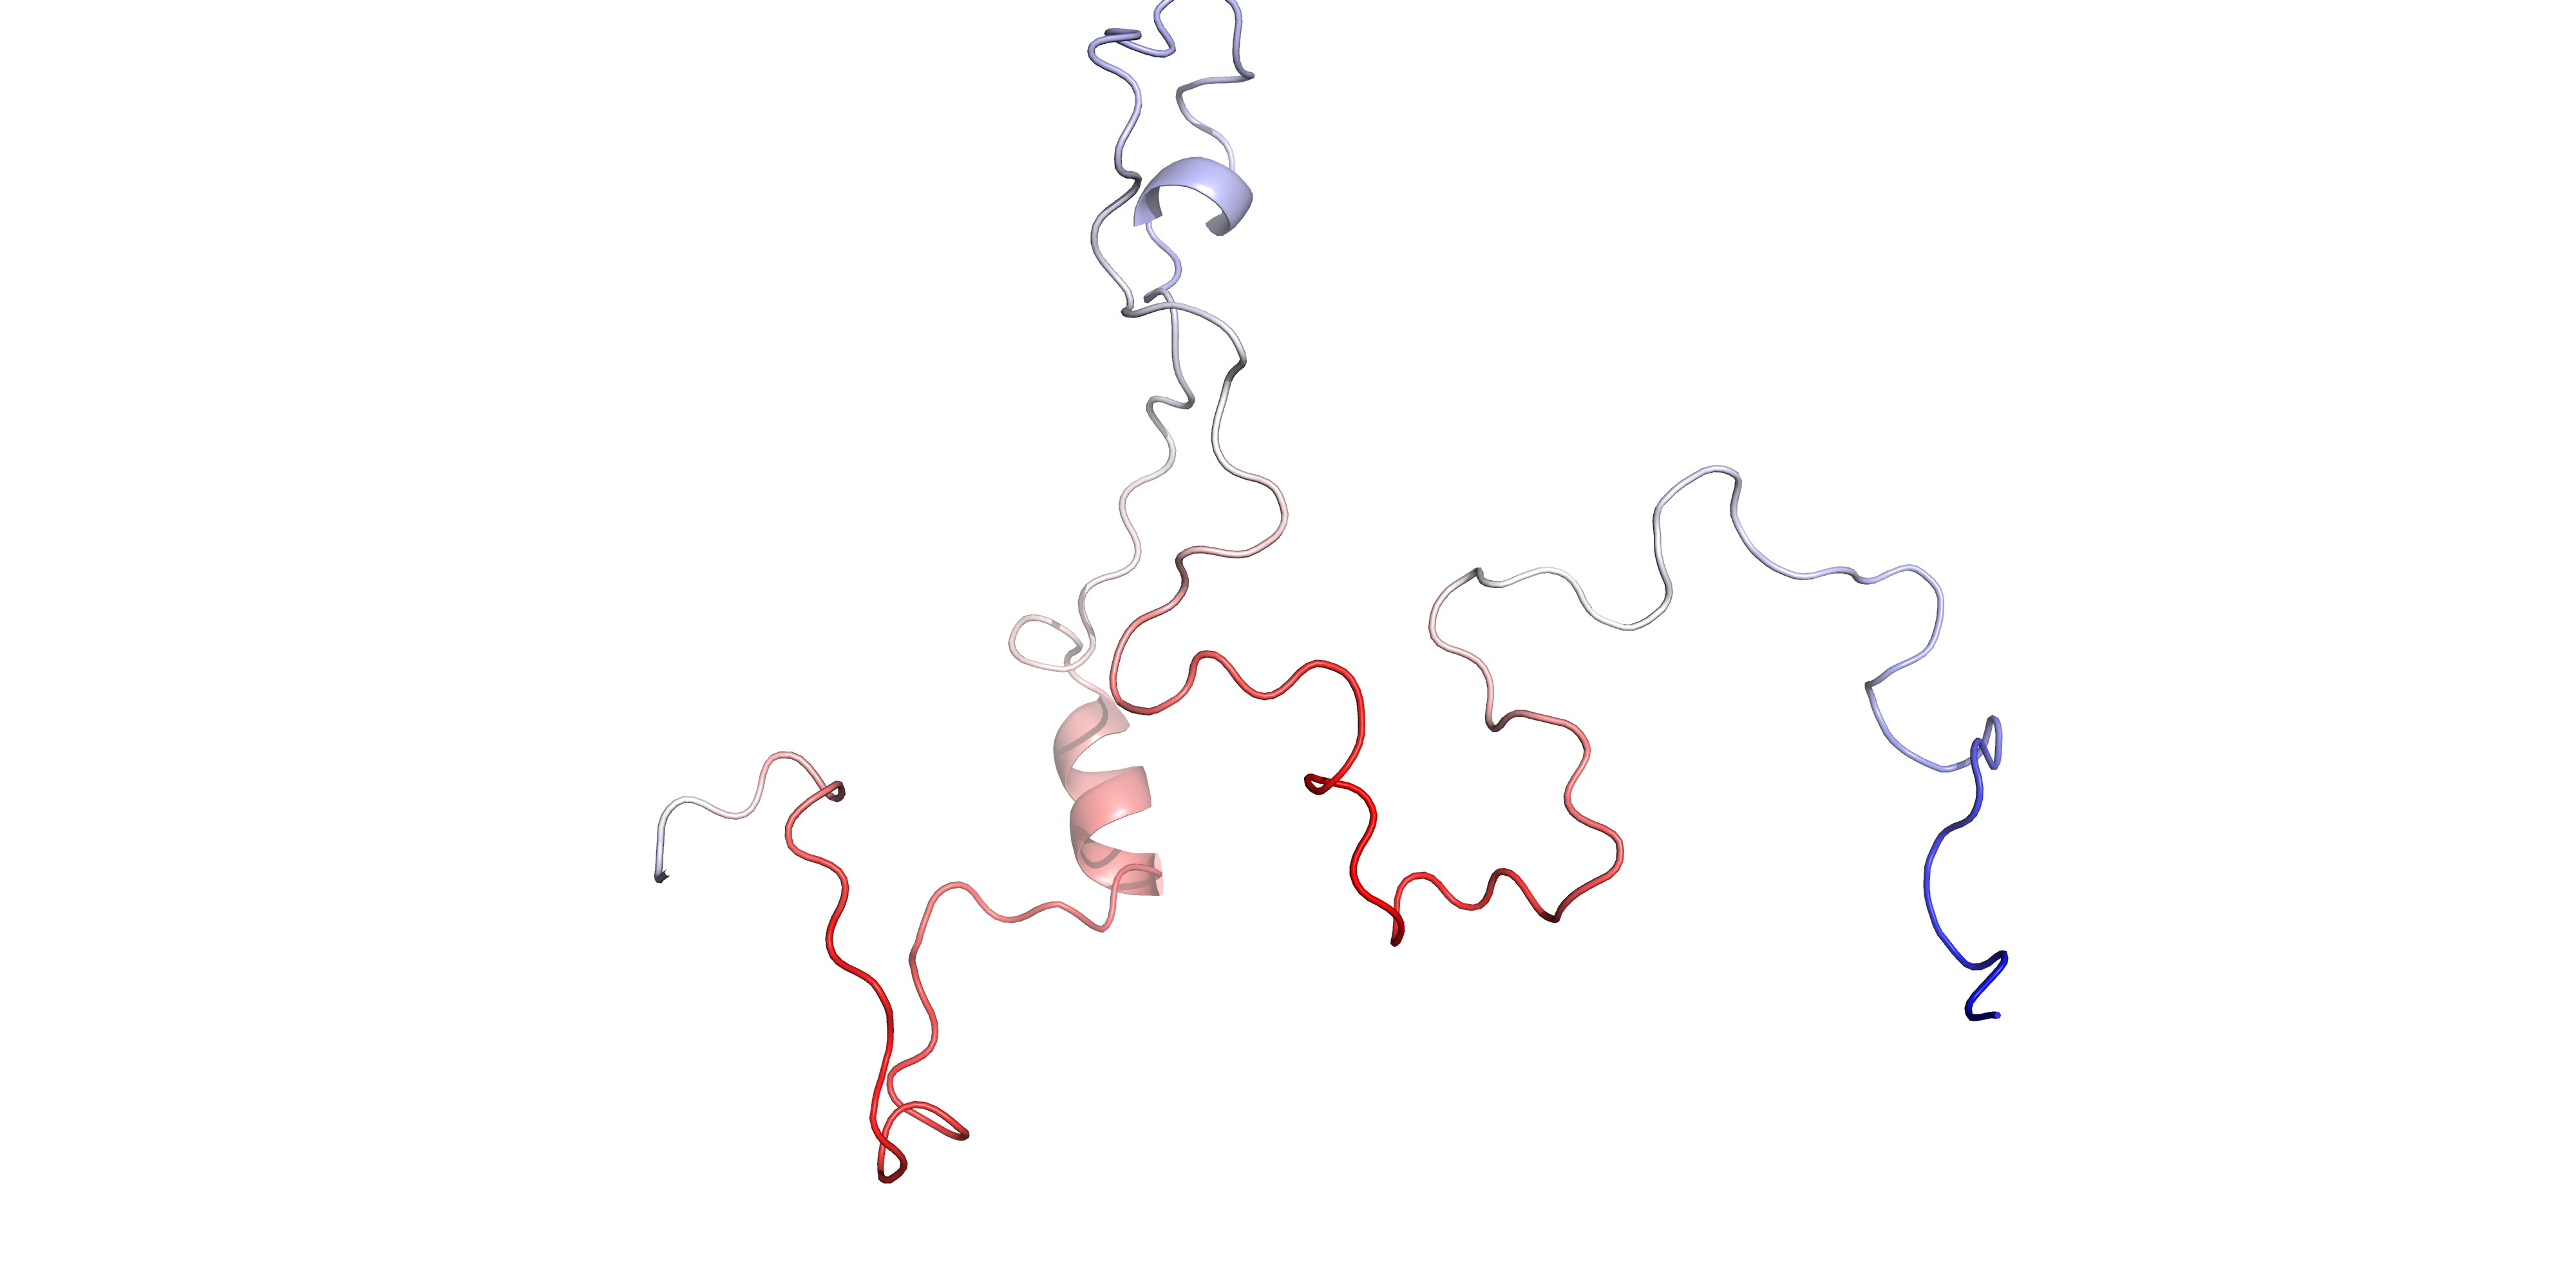
\includegraphics[width=\textwidth]{PED00020e001_pymol.png}
		\caption{Pymol image of model 001.}
		\label{model001p}
	\end{minipage}
	\begin{minipage}[b]{0.97\textwidth}
		\centering
		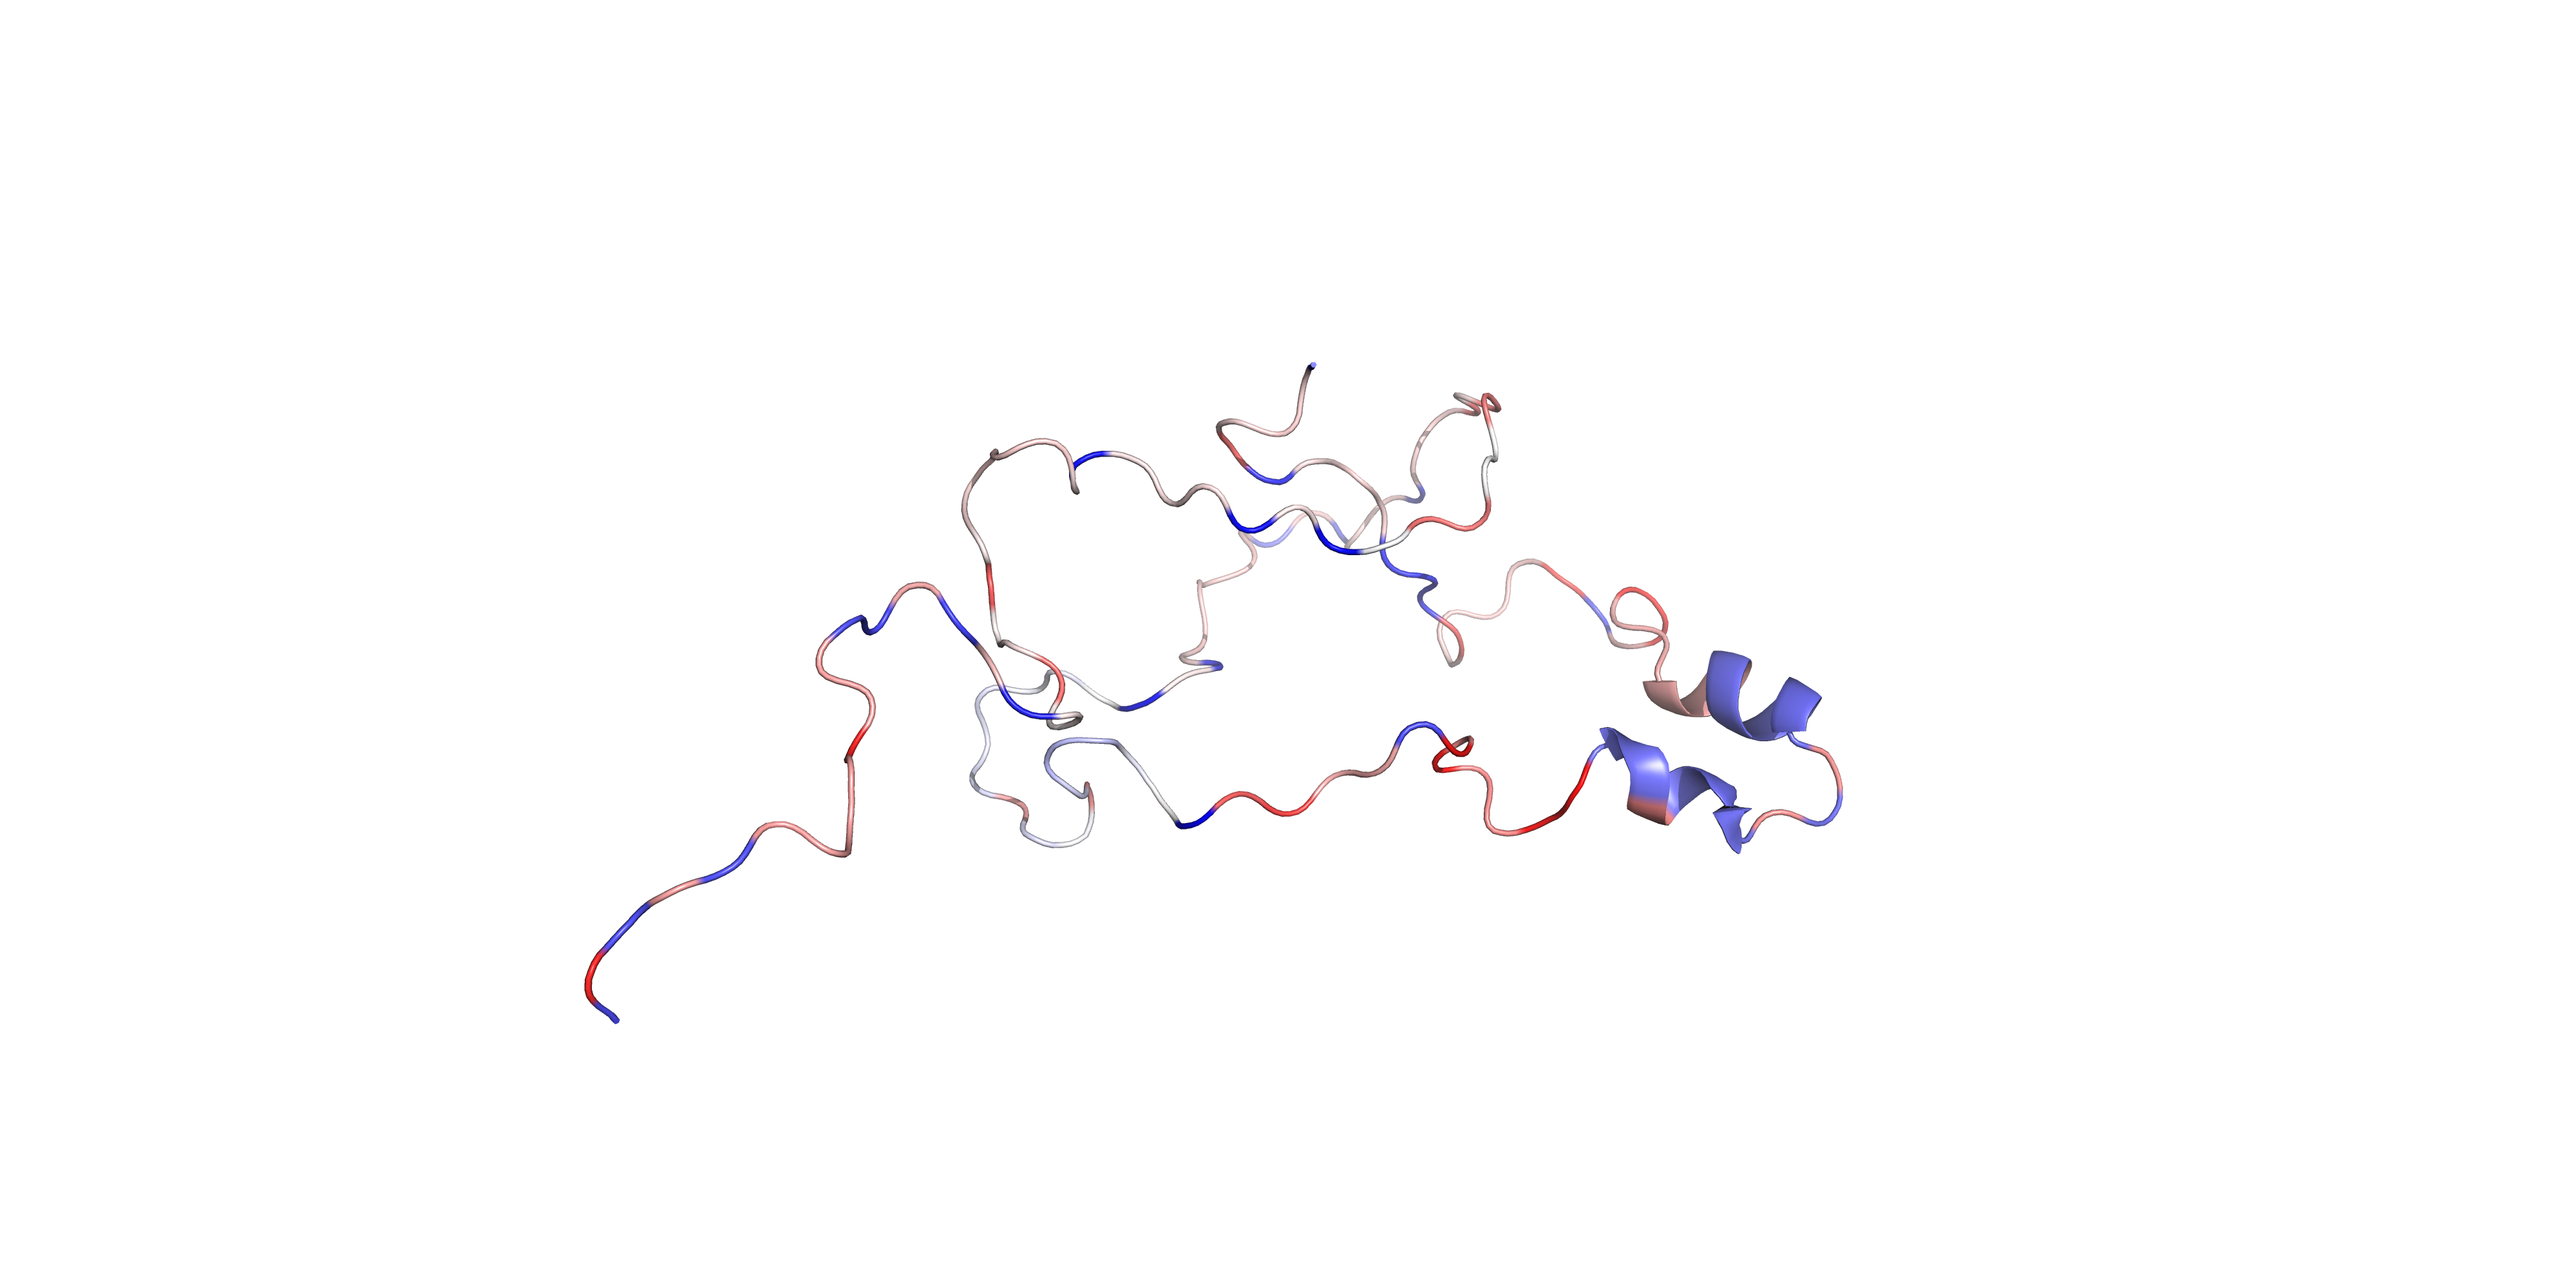
\includegraphics[width=\textwidth]{PED00020e002_pymol.png}
		\caption{Pymol image of model 002.}
		\label{model002p}
	\end{minipage}
\end{figure}
\begin{figure}[H]
	\begin{minipage}[b]{0.99\textwidth}
		\centering
		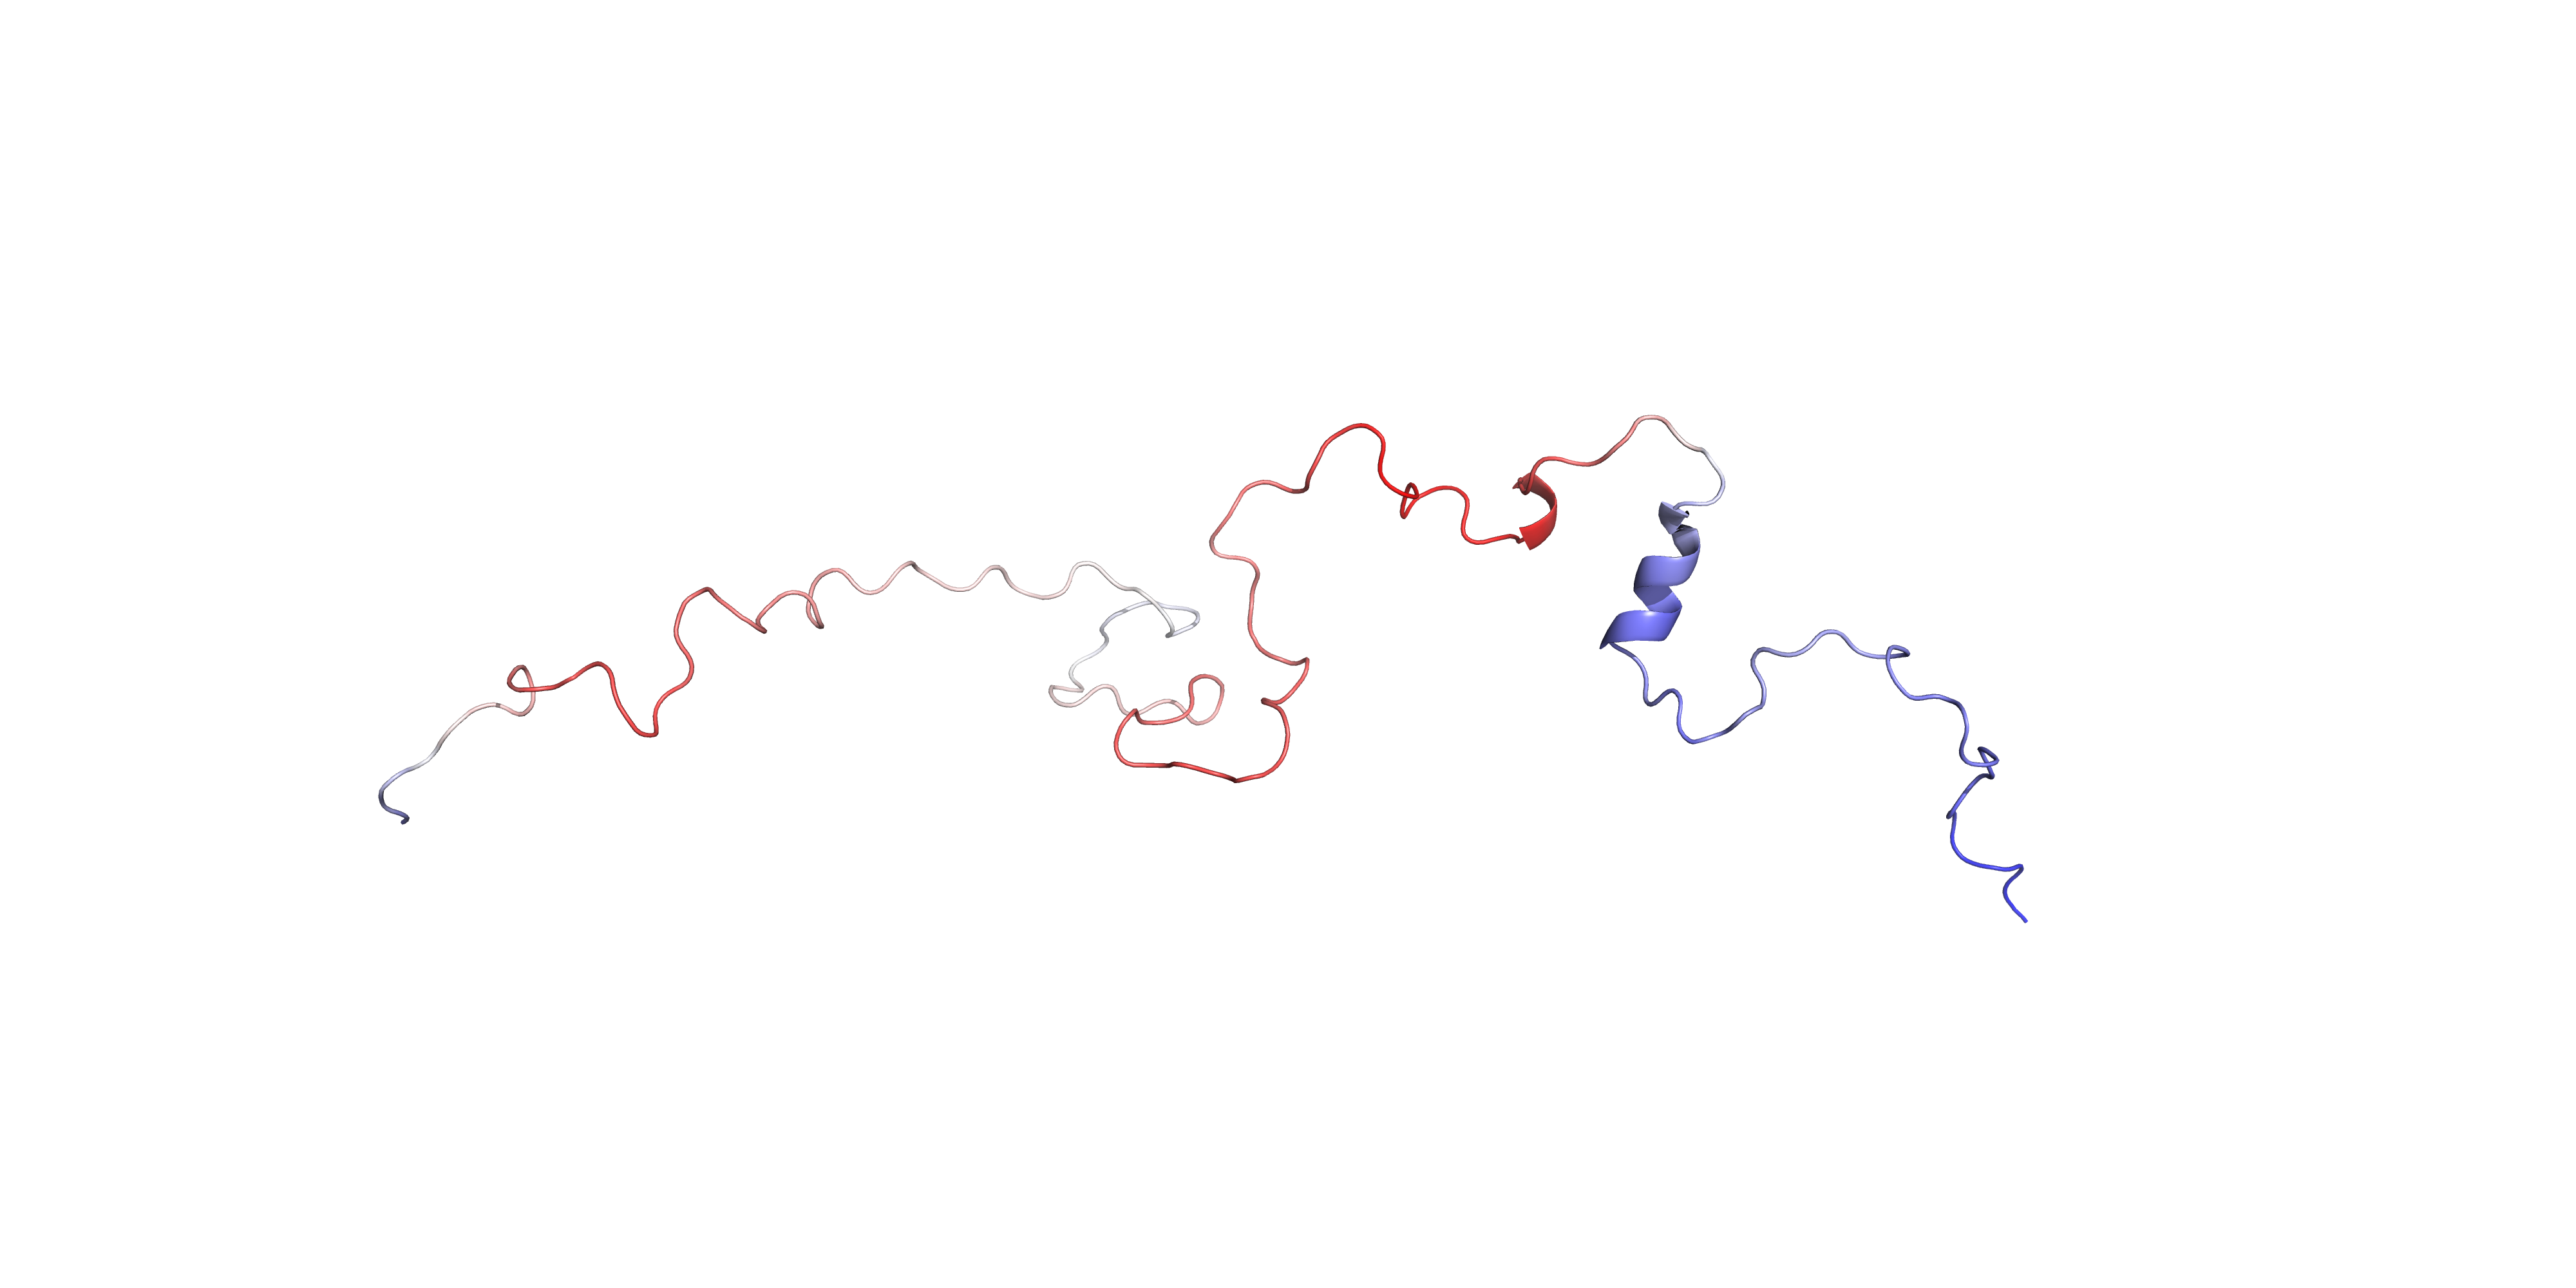
\includegraphics[width=\textwidth]{PED00020e003_pymol.png}
		\caption{Pymol image of model 003.}
		\label{model003p}
	\end{minipage}
	\begin{minipage}[b]{0.99\textwidth}
		\centering
		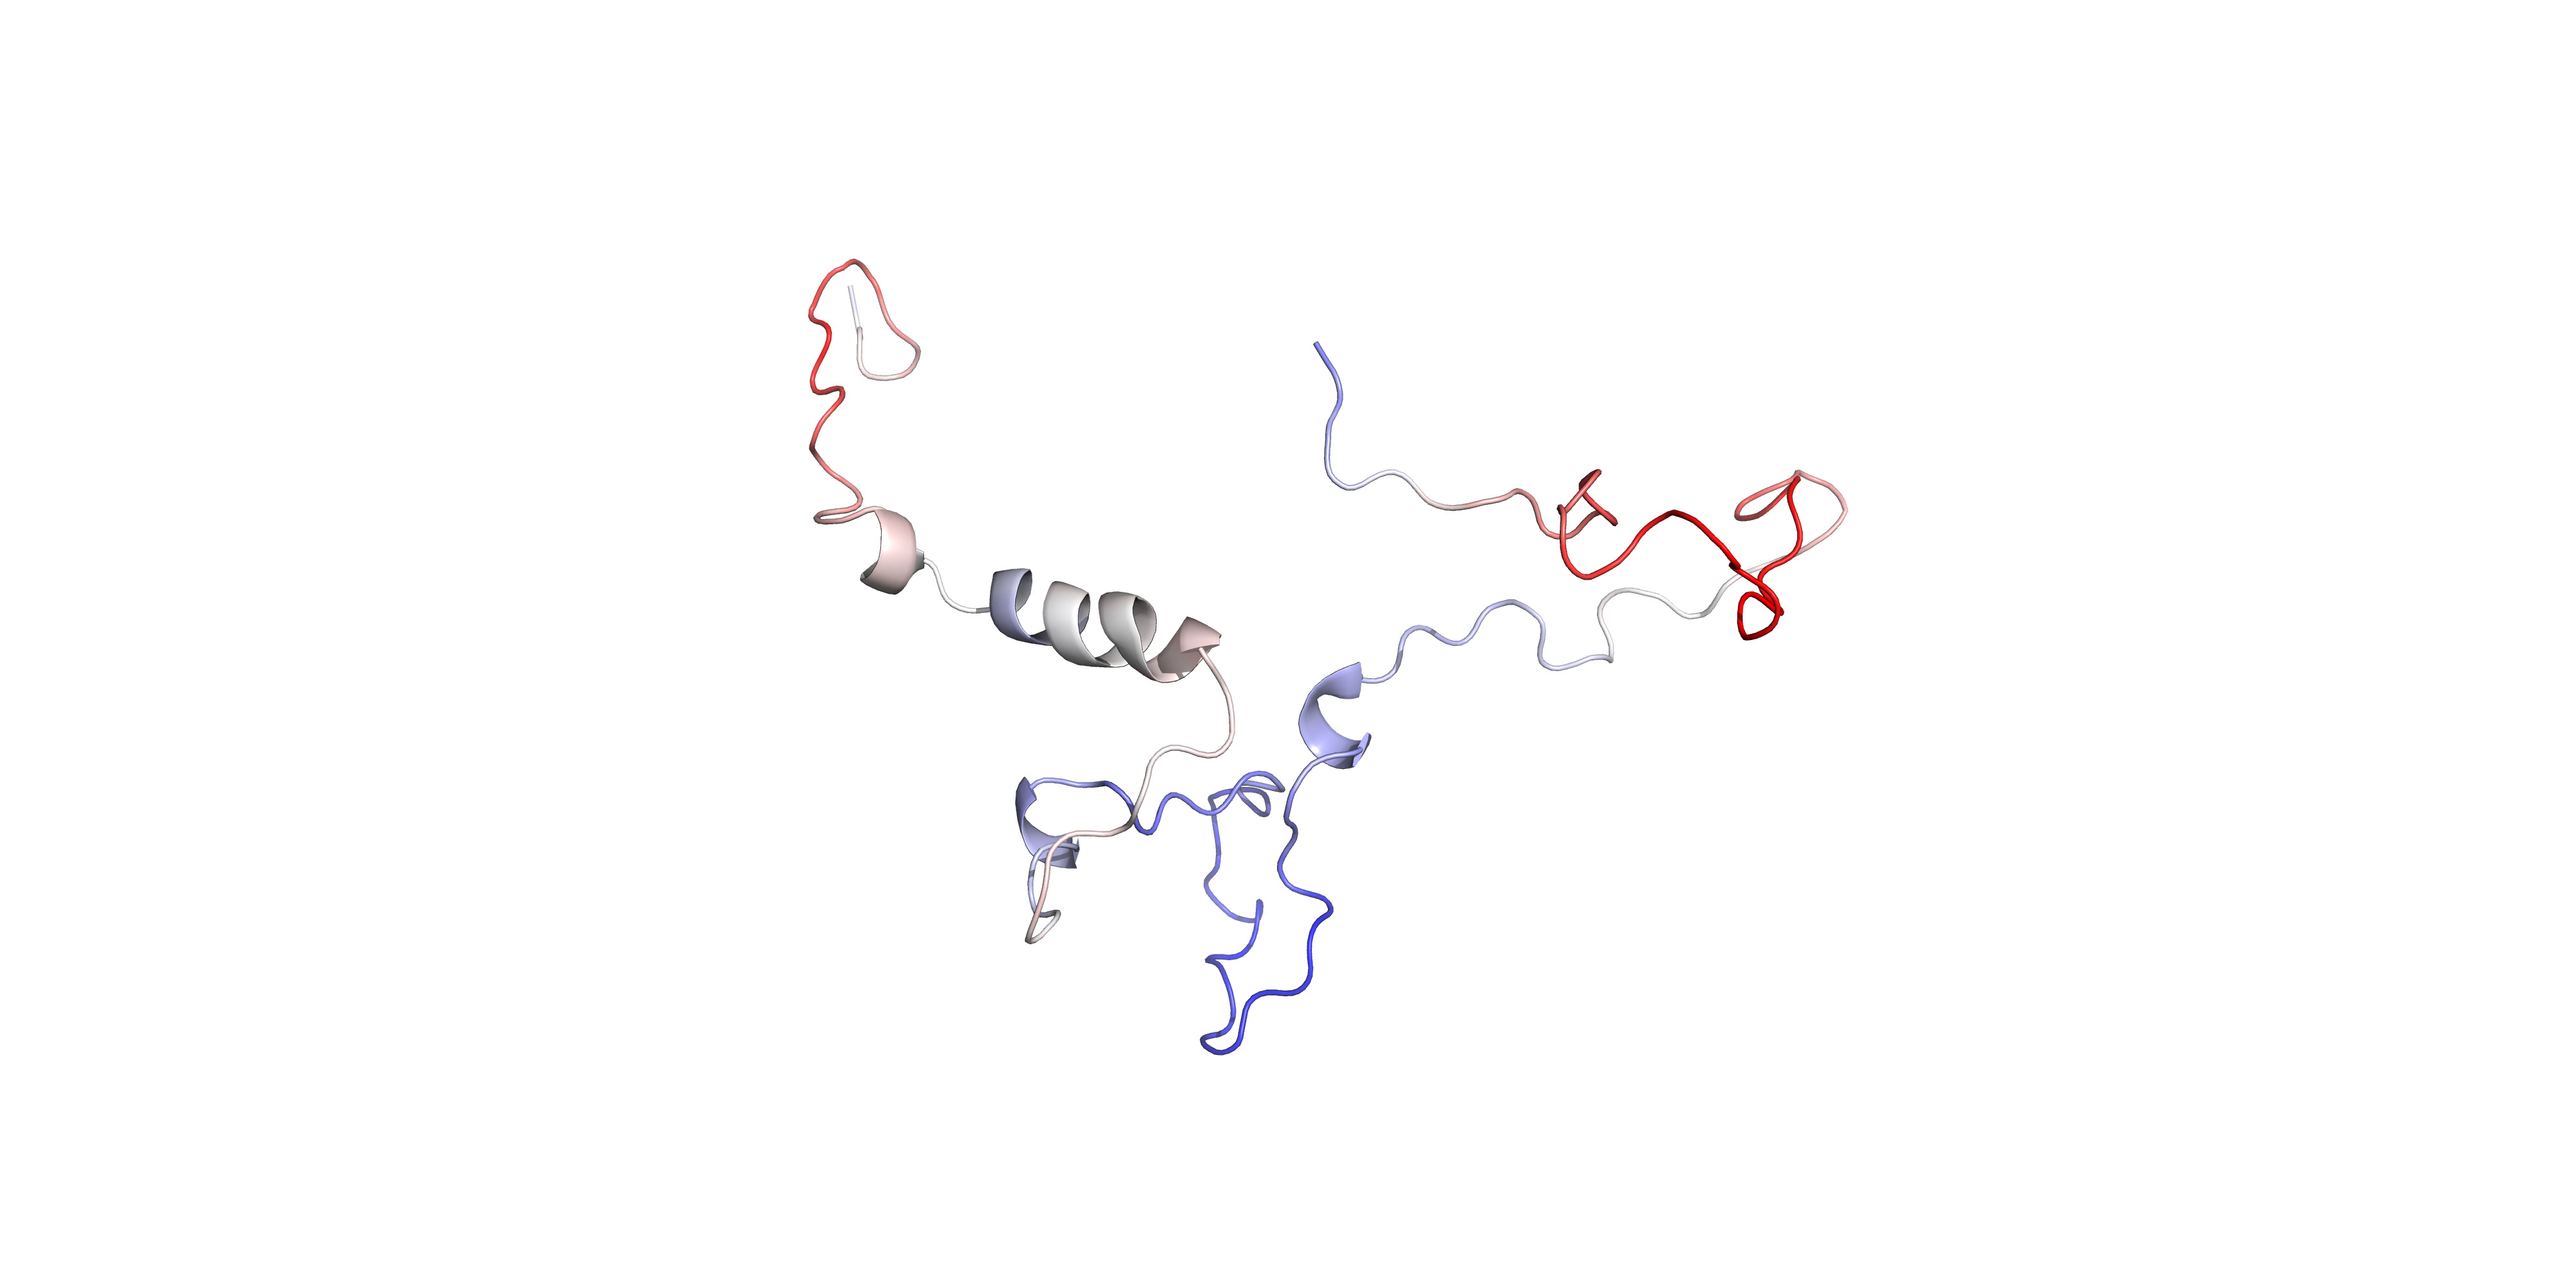
\includegraphics[width=\textwidth]{PED00020e004_pymol.png}
		\caption{Pymol image of model 004.}
		\label{model004p}
	\end{minipage}
	\begin{minipage}[b]{0.99\textwidth}
		\centering
		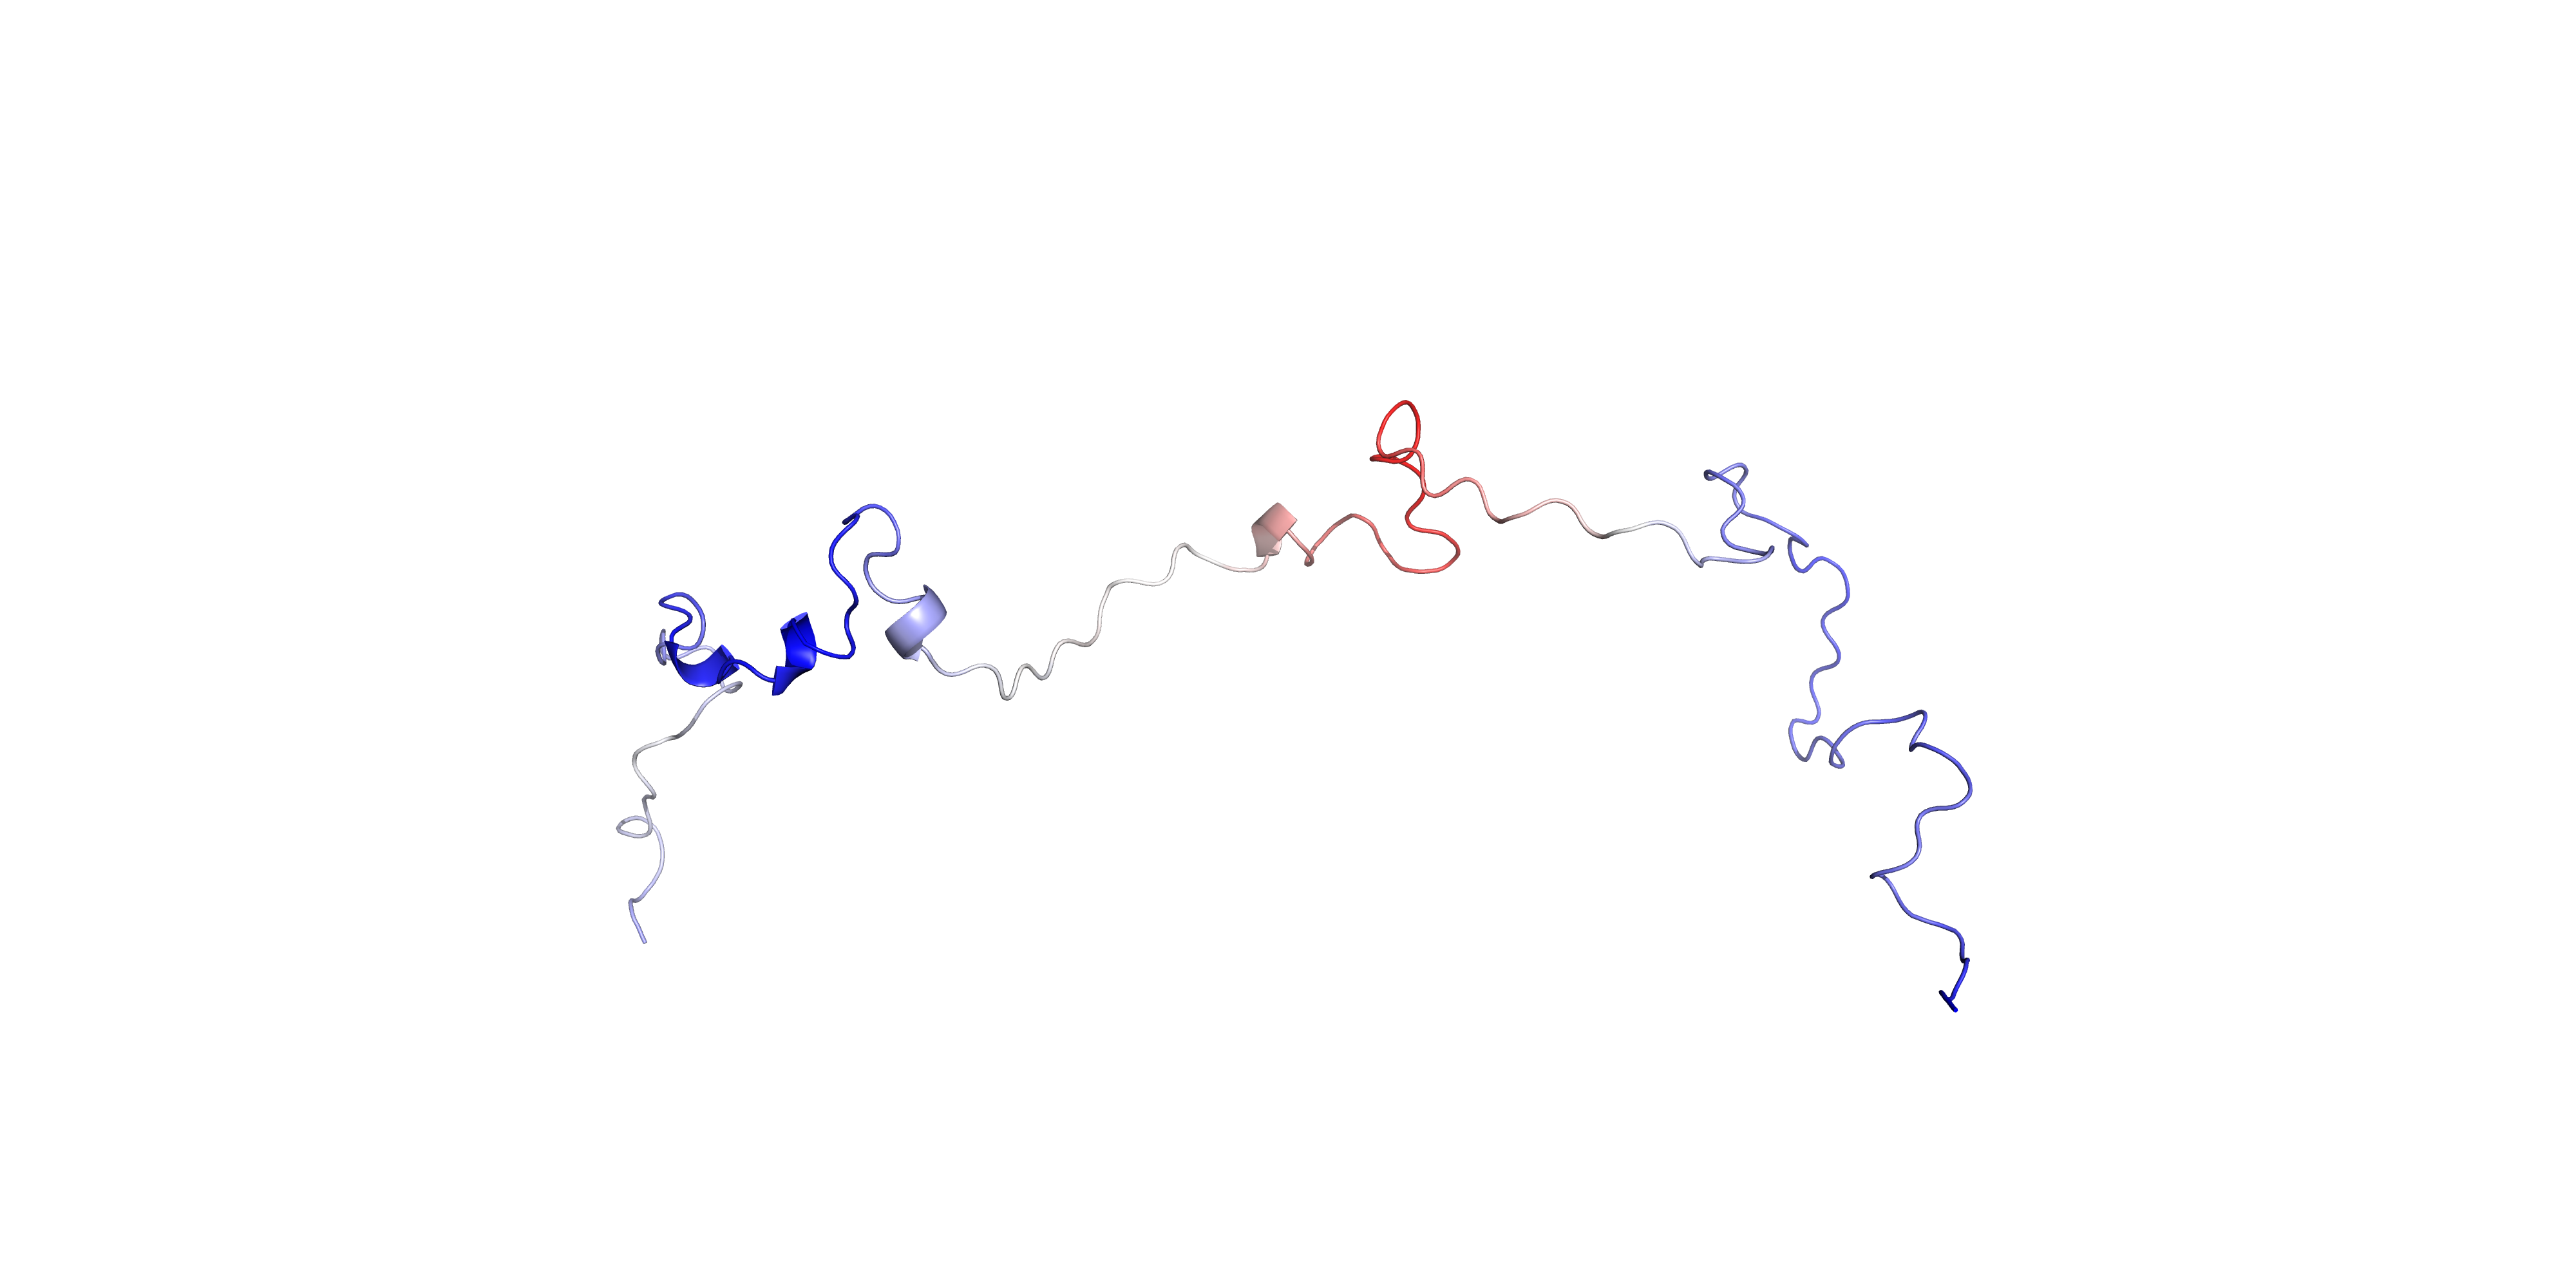
\includegraphics[width=\textwidth]{PED00020e005_pymol.png}
		\caption{Pymol image of model 005.}
		\label{model005p}
	\end{minipage}
\end{figure}

\medskip
\medskip
To understand the color variability in pymol images, here a brief description. Red identifies the residues in the structure with high variability with respect to the features considered. Blue the most stable areas. Also intermediate scenarios are displayed with color shades of red or blue.  

\medskip
Looking at figures \ref{model001p}, \ref{model002p}, \ref{model003p}, \ref{model004p} and \ref{model005p}, it is possible to see that the visualized structures are very disordered, in general. Due to the entropic high cost of folding, the well-defined structures (e.g. alpha-helix) are not many. 
